\documentclass[11pt]{amsart}
\usepackage{color}
\usepackage{color}
\usepackage{tikz}
\usetikzlibrary{decorations.markings, hobby, knots}
\usepackage{pgffor}

\begin{document}

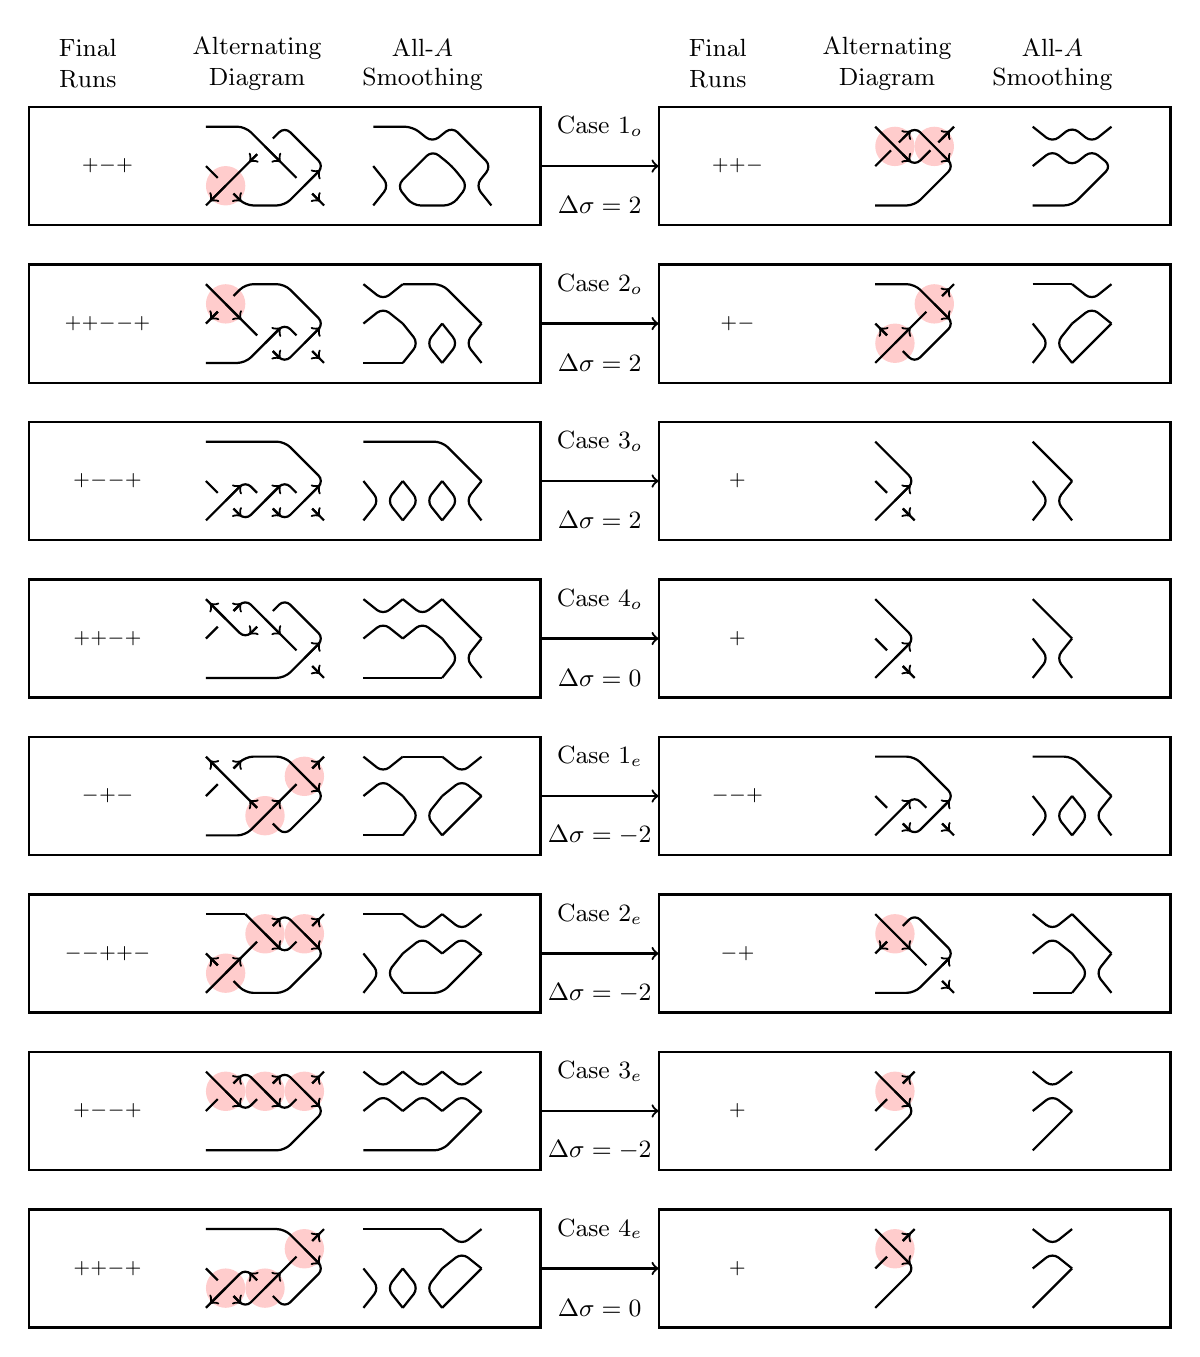
\begin{tikzpicture}[thick]

%% Odd c first

%% Case 1

\draw (-.25,1.5) node{\small{Final}};
\draw (-.25,1.1) node{\small{Runs}};

\draw (1.9,1.5) node{\small{Alternating}};
\draw (1.9,1.1) node{\small{Diagram}};

\draw (4,1.5) node{\small{All-$A$}};
\draw (4,1.1) node{\small{Smoothing}};

\draw(-1,-.75) rectangle (5.5,.75);
\draw(0,0) node{${\scriptstyle +-+}$};
\begin{scope}[scale=.5, rounded corners = 1mm, xshift = 2.5cm, yshift = -1cm]

\fill[white!80!red] (.5,.5) circle (.5cm);

\draw (0,0) -- (1.3, 1.3);
\draw (0,1) -- (.3,.7);
\draw (.7,.3) -- (1,0) -- (2,0) -- (3,1) -- (2,2) -- (1.7,1.7);
\draw (0,2) -- (1,2) -- (2.3,.7);
\draw (2.7,.3) -- (3,0);

\draw[thick,->] (.5, .5) -- (.1,.1);
\draw[thick,->] (.7,.3) -- (.9,.1);
\draw[->] (2.5, .5) -- (2.9,.9);
\draw[->] (2.7,.3) -- (2.9,.1);
\draw[->] (1.5, 1.5) -- (1.9,1.1);
\draw[->] (1.3,1.3) -- (1.1,1.1);

\end{scope}

\begin{scope}[scale=.5, rounded corners = 1mm, xshift = 6.75cm, yshift = -1cm]

\draw[-] (0,1) -- (.4,.5) -- (0,0);
\draw[-] (0,2) -- (1,2) -- (1.5,1.6) -- (2,2) -- (3,1) -- (2.6,.5) -- (3,0);

\draw[-] (1.5,1.4) -- (.6,.5) -- (1,0) -- (2,0) -- (2.4,.5) -- (2,1) -- cycle;

\end{scope}

\draw[->] (5.5,0) -- (7,0);
\draw (6.25,.5) node{\small{Case $1_o$}};
\draw (6.25,-.5) node{\small{$\Delta\sigma = 2$}};


\begin{scope}[xshift = 8 cm]
\draw (-.25,1.5) node{\small{Final}};
\draw (-.25,1.1) node{\small{Runs}};

\draw (1.9,1.5) node{\small{Alternating}};
\draw (1.9,1.1) node{\small{Diagram}};

\draw (4,1.5) node{\small{All-$A$}};
\draw (4,1.1) node{\small{Smoothing}};
\draw(-1,-.75) rectangle (5.5,.75);
\draw(0,0) node{${\scriptstyle ++-}$};
\begin{scope}[scale=.5, rounded corners = 1mm, xshift = 3.5cm, yshift = -1cm]

\fill[white!80!red] (.5,1.5) circle (.5cm);
\fill[white!80!red] (1.5,1.5) circle (.5cm);
\draw (0,0) -- (1,0) -- (2,1) -- (1,2) -- (.6,1.6);
\draw (.4,1.4) -- (0,1);
\draw (0,2) -- (1,1) -- (1.4,1.4);
\draw (1.6,1.6) -- (2,2);
\draw[thick,->] (0.7,1.7) -- (.9,1.9);
\draw[thick,->] (.7,1.3) -- (.9,1.1);
\draw[thick,->] (1.7,1.7) -- (1.9,1.9);
\draw[thick,->] (1.7, 1.3) -- (1.9,1.1);

\end{scope}

\begin{scope}[scale=.5, rounded corners = 1mm, xshift = 7.5cm, yshift = -1cm]

\draw[-] (0,2) -- (.5,1.6) -- (1,2) -- (1.5,1.6) -- (2,2);
\draw[-] (0,1) -- (.5, 1.4) -- (1,1) -- (1.5,1.4) -- (2,1) -- (1,0) -- (0,0);

\end{scope}
\end{scope}

%% Case 2
\begin{scope}[yshift = -2cm]


\draw(-1,-.75) rectangle (5.5,.75);
\draw(0,0) node{${\scriptstyle ++--+}$};
\begin{scope}[scale=.5, rounded corners = 1mm, xshift = 2.5cm, yshift = -1cm]

\fill[white!80!red] (.5,1.5) circle (.5cm);
\draw (0,0) -- (1,0) -- (2,1) -- (2.3,.7);
\draw (2.7,.3) -- (3,0);
\draw (0,1) -- (.3,1.3);
\draw (0,2) -- (1.3,.7);
\draw (1.7,.3) -- (2,0) -- (3,1) -- (2,2) -- (1,2) -- (.7,1.7);
\draw[->] (.3,1.3) -- (.1,1.1);
\draw[->] (.5,1.5) -- (.9,1.1);
\draw[->] (1.5,.5) -- (1.9,.9);
\draw[->] (1.7,.3) -- (1.9,.1);
\draw[->] (2.5,.5) -- (2.9,.9);
\draw[->] (2.7,.3) -- (2.9,.1);

\end{scope}

\begin{scope}[scale=.5, rounded corners = 1mm, xshift = 5.5cm, yshift = -1cm]

    \foreach \i/\j in {1/1} {
        \draw (\i,\j+1) -- (\i+.5,\j+.6) -- (\i+1,\j+1);
        \draw (\i,\j)   -- (\i+.5,\j+.4) -- (\i+1,\j);
    }
    \foreach \i/\j in {2/0,3/0} {
        \draw (\i,\j)   -- (\i+.4,\j+.5) -- (\i,\j+1);
        \draw (\i+1,\j) -- (\i+.6,\j+.5) -- (\i+1,\j+1);
    }
\draw (1,0) -- (2,0);
\draw (2,2) -- (3,2) -- (4,1);
\end{scope}

\draw[->] (5.5,0) -- (7,0);
\draw (6.25,.5) node{\small{Case $2_o$}};
\draw (6.25,-.5) node{\small{$\Delta\sigma = 2$}};

\end{scope}

\begin{scope}[xshift = 8cm, yshift=-2cm]

\draw(-1,-.75) rectangle (5.5,.75);

\draw(0,0) node{${\scriptstyle +-}$};
\begin{scope}[scale=.5, rounded corners = 1mm, xshift = 3.5cm, yshift = -1cm]

\fill[white!80!red] (.5,.5) circle (.5cm);
\fill[white!80!red] (1.5,1.5) circle (.5cm);
\draw (0,0) -- (1.3,1.3);
\draw (1.7,1.7)--(2,2);
\draw (0,1) -- (0.3,0.7);
\draw (0.7,0.3) -- (1,0) -- (2,1) -- (1,2) -- (0,2);

\draw[thick,->] (0.5,0.5) -- (0.9, 0.9);
\draw[thick,->] (0.3,0.7) -- (0.1,0.9);
\draw[thick,->] (1.5,1.5) -- (1.9,1.1);
\draw[thick,->] (1.7, 1.7) -- (1.9, 1.9);

\end{scope}

\begin{scope}[scale=.5, rounded corners = 1mm, xshift = 6.5cm, yshift = -1cm]

    \foreach \i/\j in {2/1} {
        \draw (\i,\j+1) -- (\i+.5,\j+.6) -- (\i+1,\j+1);
        \draw (\i,\j)   -- (\i+.5,\j+.4) -- (\i+1,\j);
    }
    \foreach \i/\j in {1/0} {
        \draw (\i,\j)   -- (\i+.4,\j+.5) -- (\i,\j+1);
        \draw (\i+1,\j) -- (\i+.6,\j+.5) -- (\i+1,\j+1);
    }
\draw[-] (2,0)--(3,1);
\draw[-] (1,2)--(2,2);
\end{scope}
\end{scope}



%% Case 3
\begin{scope}[yshift = -4cm]

\draw(-1,-.75) rectangle (5.5,.75);
\draw(0,0) node{${\scriptstyle +--+}$};
\begin{scope}[scale=.5, rounded corners = 1mm, xshift = 2.5cm, yshift = -1cm]

\draw (0,0) -- (1,1) -- (1.3,.7);
\draw (0,1) -- (.3,.7);
\draw (.7,.3) -- (1,0) -- (2,1) -- (2.3,.7);
\draw (1.7,.3) -- (2,0) -- (3,1) -- (2,2) -- (0,2);
\draw (2.7,.3) -- (3,0);
\draw[->] (0.5,0.5) -- (0.9,0.9);
\draw[->] (0.7,0.3) -- (0.9, 0.1);
\draw[->] (1.5,0.5) -- (1.9,0.9);
\draw[->] (1.7,0.3) -- (1.9, 0.1);
\draw[->] (2.5,0.5) -- (2.9,0.9);
\draw[->] (2.7,0.3) -- (2.9, 0.1);
\end{scope}

\begin{scope}[scale=.5, rounded corners = 1mm, xshift = 6.5cm, yshift = -1cm]
    \foreach \i/\j in {0/0,1/0,2/0} {
        \draw (\i,\j)   -- (\i+.4,\j+.5) -- (\i,\j+1);
        \draw (\i+1,\j) -- (\i+.6,\j+.5) -- (\i+1,\j+1);
    }
\draw (0,2) -- (2,2) -- (3,1);
\end{scope}

\draw[->] (5.5,0) -- (7,0);
\draw (6.25,.5) node{\small{Case $3_o$}};
\draw (6.25,-.5) node{\small{$\Delta\sigma = 2$}};

\end{scope}

\begin{scope}[xshift = 8cm, yshift = -4cm]

\draw(-1,-.75) rectangle (5.5,.75);

\draw(0,0) node{${\scriptstyle +}$};
\begin{scope}[scale=.5, rounded corners = 1mm, xshift = 3.5cm, yshift = -1cm]

\draw (0,1) -- (.3,.7);
\draw (.7,.3) -- (1,0);
\draw (0,0) -- (1,1) -- (0,2);

\draw[->] (.5,.5) -- (.9,.9);
\draw[->] (.7,.3) -- (.9,.1);

\end{scope}

\begin{scope}[scale=.5, rounded corners = 1mm, xshift = 7.5cm, yshift = -1cm]
    \foreach \i/\j in {0/0} {
        \draw (\i,\j)   -- (\i+.4,\j+.5) -- (\i,\j+1);
        \draw (\i+1,\j) -- (\i+.6,\j+.5) -- (\i+1,\j+1);
    }
\draw (0,2) -- (1,1);
\end{scope}
\end{scope}


%% Case 4
\begin{scope}[yshift = -6cm]

\draw(-1,-.75) rectangle (5.5,.75);
\draw(0,0) node{${\scriptstyle ++-+}$};
\begin{scope}[scale=.5, rounded corners = 1mm, xshift = 2.5cm, yshift = -1cm]
\draw (0,0) -- (2,0) -- (3,1) -- (2,2) -- (1.7,1.7);
\draw (1.3,1.3) -- (1,1) -- (0,2);
\draw (0,1) -- (.3,1.3);
\draw (.7,1.7) -- (1,2) -- (2.3,.7);
\draw (2.7,0.3) -- (3,0);

\draw[->] (0.5, 1.5) -- (0.1, 1.9);
\draw[->] (0.7,1.7) -- (0.9,1.9);
\draw[->] (1.5, 1.5) -- (1.9,1.1);
\draw[->] (1.3,1.3) -- (1.1, 1.1);
\draw[->] (2.5,0.5) -- (2.9,0.9);
\draw[->] (2.7,0.3) -- (2.9, 0.1);
\end{scope}

\begin{scope}[scale=.5, rounded corners = 1mm, xshift = 6.5cm, yshift = -1cm]
    \foreach \i/\j in {0/1,1/1} {
        \draw (\i,\j+1) -- (\i+.5,\j+.6) -- (\i+1,\j+1);
        \draw (\i,\j)   -- (\i+.5,\j+.4) -- (\i+1,\j);
    }
    \foreach \i/\j in {2/0} {
        \draw (\i,\j)   -- (\i+.4,\j+.5) -- (\i,\j+1);
        \draw (\i+1,\j) -- (\i+.6,\j+.5) -- (\i+1,\j+1);
    }
\draw (0,0) -- (2,0);
\draw (2,2) -- (3,1);
\end{scope}
\draw[->] (5.5,0) -- (7,0);
\draw (6.25,.5) node{\small{Case $4_o$}};
\draw (6.25,-.5) node{\small{$\Delta\sigma = 0$}};

\end{scope}

\begin{scope}[xshift = 8cm, yshift = -6cm]
\draw(-1,-.75) rectangle (5.5,.75);

\draw(0,0) node{${\scriptstyle +}$};
\begin{scope}[scale=.5, rounded corners = 1mm, xshift = 3.5cm, yshift = -1cm]

\draw (0,1) -- (.3,.7);
\draw (.7,.3) -- (1,0);
\draw (0,0) -- (1,1) -- (0,2);

\draw[->] (.5,.5) -- (.9,.9);
\draw[->] (.7,.3) -- (.9,.1);

\end{scope}

\begin{scope}[scale=.5, rounded corners = 1mm, xshift = 7.5cm, yshift = -1cm]
    \foreach \i/\j in {0/0} {
        \draw (\i,\j)   -- (\i+.4,\j+.5) -- (\i,\j+1);
        \draw (\i+1,\j) -- (\i+.6,\j+.5) -- (\i+1,\j+1);
    }
\draw (0,2) -- (1,1);
\end{scope}
\end{scope}

%%%%%%%%%%%%%%%%%%%%%%%%%%%%%%%%%%%%%%%%%%%%%%%%% Even c next

%% Case 1


\begin{scope}[yshift = -8cm]

\draw(-1,-.75) rectangle (5.5,.75);
\draw(0,0) node{${\scriptstyle -+-}$};
\begin{scope}[scale=.5, rounded corners = 1mm, xshift = 2.5cm, yshift = -1cm]
\fill[white!80!red] (1.5,.5) circle (.5cm);
\fill[white!80!red] (2.5,1.5) circle (.5cm);
\draw (0,0) -- (1,0) -- (2,1) -- (2.3,1.3);
\draw (2.7,1.7) -- (3,2);
\draw (0,2) -- (1,1) -- (1.3,.7);
\draw (1.7,.3) -- (2,0) -- (3,1) -- (2,2) -- (1,2) -- (.7,1.7);
\draw (0,1) -- (.3,1.3);

\draw[->] (.3,1.7) -- (.1,1.9);
\draw[->] (.7,1.7) -- (.9,1.9);
\draw[thick, ->] (1.7,.7) -- (1.9,.9);
\draw[thick, ->] (1.3,.7) -- (1.1,.9);
\draw[thick,->] (2.7,1.7) -- (2.9,1.9);
\draw[thick,->] (2.7,1.3) -- (2.9,1.1);

\end{scope}



\begin{scope}[scale=.5, rounded corners = 1mm, xshift = 6.5cm, yshift = -1cm]
    \foreach \i/\j in {0/1,2/1} {
        \draw (\i,\j+1) -- (\i+.5,\j+.6) -- (\i+1,\j+1);
        \draw (\i,\j)   -- (\i+.5,\j+.4) -- (\i+1,\j);
    }
    \foreach \i/\j in {1/0} {
        \draw (\i,\j)   -- (\i+.4,\j+.5) -- (\i,\j+1);
        \draw (\i+1,\j) -- (\i+.6,\j+.5) -- (\i+1,\j+1);
    }
\draw (0,0)--(1,0);
\draw (1,2)--(2,2);
\draw (2,0)--(3,1);
\end{scope}


\draw[->] (5.5,0) -- (7,0);
\draw (6.25,.5) node{\small{Case $1_e$}};
\draw (6.25,-.5) node{\small{$\Delta\sigma = -2$}};


\begin{scope}[xshift = 8 cm]
\draw(-1,-.75) rectangle (5.5,.75);
\draw(0,0) node{${\scriptstyle -{}-+}$};
\begin{scope}[scale=.5, rounded corners = 1mm, xshift = 3.5cm, yshift = -1cm]
\draw (0,2) -- (1,2) -- (2,1) -- (1,0) -- (.7,.3);
\draw (.3,.7) -- (0,1);
\draw (0,0) -- (1,1) -- (1.3,.7);
\draw (1.7,.3) -- (2,0);
\draw[->] (0.7,.3) -- (.9,.1);
\draw[->] (.7,.7) -- (.9,.9);
\draw[->] (1.7,.3) -- (1.9,.1);
\draw[->] (1.7, .7) -- (1.9,.9);

\end{scope}

\begin{scope}[scale=.5, rounded corners = 1mm, xshift = 7.5cm, yshift = -1cm]

    \foreach \i/\j in {0/0,1/0} {
        \draw (\i,\j)   -- (\i+.4,\j+.5) -- (\i,\j+1);
        \draw (\i+1,\j) -- (\i+.6,\j+.5) -- (\i+1,\j+1);
    }
\draw (0,2) -- (1,2) -- (2,1);
\end{scope}
\end{scope}
\end{scope}

%% Case 2 even
\begin{scope}[yshift = -10cm]


\draw(-1,-.75) rectangle (5.5,.75);
\draw(0,0) node{${\scriptstyle -{}-++-}$};
\begin{scope}[scale=.5, rounded corners = 1mm, xshift = 2.5cm, yshift = -1cm]

\fill[white!80!red] (.5,.5) circle (.5cm);
\fill[white!80!red] (1.5,1.5) circle (.5cm);
\fill[white!80!red] (2.5,1.5) circle (.5cm);
\draw (1,2) -- (2,1) -- (2.3,1.3);
\draw (2.7,1.7) -- (3,2);
\draw (0,1) -- (.3,.7);
\draw (0,0) -- (1.3,1.3);
\draw (1.7,1.7) -- (2,2) -- (3,1) -- (2,0) -- (1,0) -- (.7,.3);
\draw[thick,->] (.3,.7) -- (.1,.9);
\draw[thick,->] (.5,.5) -- (.9,.9);
\draw[thick,->] (1.5,1.5) -- (1.9,1.1);
\draw[thick,->] (1.7,1.7) -- (1.9,1.9);
\draw[thick,->] (2.5,1.5) -- (2.9,1.1);
\draw[thick,->] (2.7,1.7) -- (2.9,1.9);
\draw (0,2) -- (1,2);
\end{scope}

\begin{scope}[scale=.5, rounded corners = 1mm, xshift = 5.5cm, yshift = -1cm]

    \foreach \i/\j in {2/1,3/1} {
        \draw (\i,\j+1) -- (\i+.5,\j+.6) -- (\i+1,\j+1);
        \draw (\i,\j)   -- (\i+.5,\j+.4) -- (\i+1,\j);
    }
    \foreach \i/\j in {1/0} {
        \draw (\i,\j)   -- (\i+.4,\j+.5) -- (\i,\j+1);
        \draw (\i+1,\j) -- (\i+.6,\j+.5) -- (\i+1,\j+1);
    }
\draw (1,2) -- (2,2);
\draw (2,0) -- (3,0) -- (4,1);
\end{scope}

\draw[->] (5.5,0) -- (7,0);
\draw (6.25,.5) node{\small{Case $2_e$}};
\draw (6.25,-.5) node{\small{$\Delta\sigma = -2$}};
\end{scope}

\begin{scope}[xshift = 8cm, yshift=-10cm]

\draw(-1,-.75) rectangle (5.5,.75);

\draw(0,0) node{${\scriptstyle -+}$};
\begin{scope}[scale=.5, rounded corners = 1mm, xshift = 3.5cm, yshift = -1cm]

\fill[white!80!red] (.5,1.5) circle (.5cm);
\draw (0,2) -- (1.3,.7);
\draw (1.7,.3)--(2,0);
\draw (0,1) -- (0.3,1.3);
\draw (0.7,1.7) -- (1,2) -- (2,1) -- (1,0) -- (0,0);


\draw[->] (0.3,1.3) -- (0.1, 1.1);
\draw[->] (0.7,1.3) -- (0.9,1.1);
\draw[->] (1.7,0.7) -- (1.9,0.9);
\draw[->] (1.7, 0.3) -- (1.9, 0.1);

\end{scope}

\begin{scope}[scale=.5, rounded corners = 1mm, xshift = 6.5cm, yshift = -1cm]

    \foreach \i/\j in {1/1} {
        \draw (\i,\j+1) -- (\i+.5,\j+.6) -- (\i+1,\j+1);
        \draw (\i,\j)   -- (\i+.5,\j+.4) -- (\i+1,\j);
    }
    \foreach \i/\j in {2/0} {
        \draw (\i,\j)   -- (\i+.4,\j+.5) -- (\i,\j+1);
        \draw (\i+1,\j) -- (\i+.6,\j+.5) -- (\i+1,\j+1);
    }
\draw[-] (2,2) -- (3,1);
\draw[-] (1,0)--(2,0);
\end{scope}
\end{scope}



%% Case 3 even
\begin{scope}[yshift = -12cm]

\draw(-1,-.75) rectangle (5.5,.75);
\draw(0,0) node{${\scriptstyle +--+}$};
\begin{scope}[scale=.5, rounded corners = 1mm, xshift = 2.5cm, yshift = -1cm]

\fill[white!80!red] (.5,1.5) circle (.5cm);
\fill[white!80!red] (1.5,1.5) circle (.5cm);
\fill[white!80!red] (2.5,1.5) circle (.5cm);
\draw (0,2) -- (1,1) -- (1.3,1.3);
\draw (0,1) -- (.3,1.3);
\draw (.7,1.7) -- (1,2) -- (2,1) -- (2.3,1.3);
\draw (1.7,1.7) -- (2,2) -- (3,1) -- (2,0) -- (0,0);
\draw (2.7,1.7) -- (3,2);
\draw[thick,->] (0.5,1.5) -- (0.9,1.1);
\draw[thick,->] (0.7,1.7) -- (0.9,1.9);
\draw[thick,->] (1.5,1.5) -- (1.9,1.1);
\draw[thick,->] (1.7,1.7) -- (1.9,1.9);
\draw[thick,->] (2.5,1.5) -- (2.9,1.1);
\draw[thick,->] (2.7,1.7) -- (2.9,1.9);
\end{scope}

\begin{scope}[scale=.5, rounded corners = 1mm, xshift = 6.5cm, yshift = -1cm]
    \foreach \i/\j in {0/1,1/1,2/1} {
        \draw (\i,\j+1) -- (\i+.5,\j+.6) -- (\i+1,\j+1);
        \draw (\i,\j)   -- (\i+.5,\j+.4) -- (\i+1,\j);
    }
\draw (0,0) -- (2,0) -- (3,1);
\end{scope}

\draw[->] (5.5,0) -- (7,0);
\draw (6.25,.5) node{\small{Case $3_e$}};
\draw (6.25,-.5) node{\small{$\Delta\sigma = -2$}};

\end{scope}

\begin{scope}[xshift = 8cm, yshift = -12cm]

\draw(-1,-.75) rectangle (5.5,.75);

\draw(0,0) node{${\scriptstyle +}$};
\begin{scope}[scale=.5, rounded corners = 1mm, xshift = 3.5cm, yshift = -1cm]

\fill[white!80!red] (.5,1.5) circle (.5cm);
\draw (0,1) -- (.3,1.3);
\draw (.7,1.7) -- (1,2);
\draw (0,2) -- (1,1) -- (0,0);

\draw[thick,->] (.5,1.5) -- (.9,1.1);
\draw[thick,->] (.7,1.7) -- (.9,1.9);

\end{scope}

\begin{scope}[scale=.5, rounded corners = 1mm, xshift = 7.5cm, yshift = -1cm]
    \foreach \i/\j in {0/1} {
        \draw (\i,\j+1) -- (\i+.5,\j+.6) -- (\i+1,\j+1);
        \draw (\i,\j)   -- (\i+.5,\j+.4) -- (\i+1,\j);
    }
\draw (0,0) -- (1,1);
\end{scope}
\end{scope}


%% Case 4
\begin{scope}[yshift = -14cm]

\draw(-1,-.75) rectangle (5.5,.75);
\draw(0,0) node{${\scriptstyle ++-+}$};
\begin{scope}[scale=.5, rounded corners = 1mm, xshift = 2.5cm, yshift = -1cm]
\fill[white!80!red] (.5,.5) circle (.5cm);
\fill[white!80!red] (1.5,.5) circle (.5cm);
\fill[white!80!red] (2.5,1.5) circle (.5cm);
\draw (0,2) -- (2,2) -- (3,1) -- (2,0) -- (1.7,.3);
\draw (1.3,.7) -- (1,1) -- (0,0);
\draw (0,1) -- (.3,.7);
\draw (.7,.3) -- (1,0) -- (2.3,1.3);
\draw (2.7,1.7) -- (3,2);

\draw[thick,->] (0.5,.5) -- (0.1,.1);
\draw[thick,->] (0.7,.3) -- (0.9,.1);
\draw[thick,->] (1.5,.5) -- (1.9,.9);
\draw[thick,->] (1.3,.7) -- (1.1,.9);
\draw[thick,->] (2.5,1.5) --(2.9,1.1);
\draw[thick,->] (2.7,1.7) --(2.9,1.9);
\end{scope}

\begin{scope}[scale=.5, rounded corners = 1mm, xshift = 6.5cm, yshift = -1cm]
    \foreach \i/\j in {2/1} {
        \draw (\i,\j+1) -- (\i+.5,\j+.6) -- (\i+1,\j+1);
        \draw (\i,\j)   -- (\i+.5,\j+.4) -- (\i+1,\j);
    }
    \foreach \i/\j in {0/0,1/0} {
        \draw (\i,\j)   -- (\i+.4,\j+.5) -- (\i,\j+1);
        \draw (\i+1,\j) -- (\i+.6,\j+.5) -- (\i+1,\j+1);
    }
\draw (0,2) -- (2,2);
\draw (2,0) -- (3,1);
\end{scope}
\draw[->] (5.5,0) -- (7,0);
\draw (6.25,.5) node{\small{Case $4_e$}};
\draw (6.25,-.5) node{\small{$\Delta\sigma = 0$}};

\end{scope}

\begin{scope}[xshift = 8cm, yshift = -14cm]
\draw(-1,-.75) rectangle (5.5,.75);

\draw(0,0) node{${\scriptstyle +}$};
\begin{scope}[scale=.5, rounded corners = 1mm, xshift = 3.5cm, yshift = -1cm]

\fill[white!80!red] (.5,1.5) circle (.5cm);
\draw (0,1) -- (.3,1.3);
\draw (.7,1.7) -- (1,2);
\draw (0,2) -- (1,1) -- (0,0);

\draw[thick,->] (.5,1.5) -- (.9,1.1);
\draw[thick,->] (.7,1.7) -- (.9,1.9);

\end{scope}

\begin{scope}[scale=.5, rounded corners = 1mm, xshift = 7.5cm, yshift = -1cm]
    \foreach \i/\j in {0/1} {
        \draw (\i,\j+1) -- (\i+.5,\j+.6) -- (\i+1,\j+1);
        \draw (\i,\j)   -- (\i+.5,\j+.4) -- (\i+1,\j);
    }
\draw (0,0) -- (1,1);
\end{scope}
\end{scope}



    
\end{tikzpicture}

\end{document}